%!TEX root = ../main.tex
%%%%%%%%%%%%%%%%%%%%%%%%%%%%%%%%%%
% Links:
%
% Difficulty:
% Companies: 
%%%%%%%%%%%%%%%%%%%%%%%%%%%%%%%%%%

\chapter{Delete duplicates from Linked List}
\label{ch:delete_duplicates_list}
\section*{Introduction}
This chapter deals with a fairly simple problem on linked lists that is popular during the preliminary interview stage. Given it's ubiquity, it is important to have a good understanding of the solution so that you can implement it quickly and, more importantly, flawlessly during a real interview. 
\section{Problem statement}
\begin{exercise}
Given a singly linked link $L$ (see definition at Listing \ref{list:delete_duplicates_list:linked_list}), return a linked list with no duplicates.

	\begin{example}
		\label{ex:delete_duplicates_list:example1}
		\hfill \\
		Given the input list in Figure \ref{fig:delete_duplicates_list:example1_1} the function returns the list in Figure \ref{fig:delete_duplicates_list:example1_2} 
	\end{example}

	\begin{example}
		\hfill \\
		\label{ex:delete_duplicates_list:example2}
		Given the input list in Figure \ref{fig:delete_duplicates_list:example2_1} the function returns the list in Figure \ref{fig:delete_duplicates_list:example2_2} 
	\end{example}
\end{exercise}

\begin{figure}
	\centering
	\begin{subfigure}[t]{0.45\textwidth}
		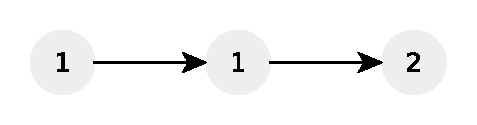
\includegraphics[width=1\linewidth]{sources/delete_duplicates_list/images/example1_1}
		\caption{Input list for Example \ref{ex:delete_duplicates_list:example1}}
		\label{fig:delete_duplicates_list:example1_1}
	 \end{subfigure}
	\hfill
	\begin{subfigure}[t]{0.45\textwidth}
		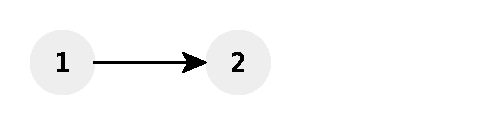
\includegraphics[width=1\linewidth]{sources/delete_duplicates_list/images/example1_2}
		\caption{List shown in Figure \ref{fig:delete_duplicates_list:example1_1} with duplicates removed.}
		\label{fig:delete_duplicates_list:example1_2}
	 \end{subfigure}
	 \hfill
	 \begin{subfigure}[t]{0.99\textwidth}
		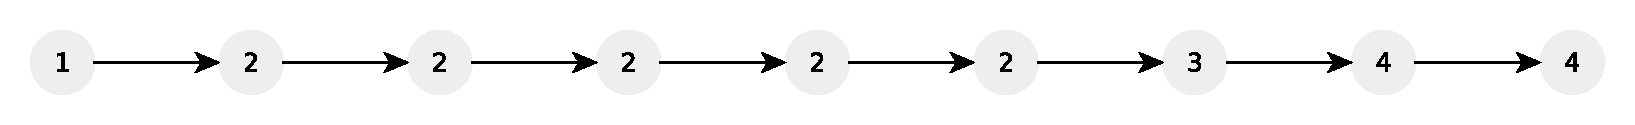
\includegraphics[width=1\linewidth]{sources/delete_duplicates_list/images/example2_1}
		\caption{Input list for Example \ref{ex:delete_duplicates_list:example2}}
		\label{fig:delete_duplicates_list:example2_1}
	 \end{subfigure}
	  \hfill
	  \begin{subfigure}[t]{0.99\textwidth}
		  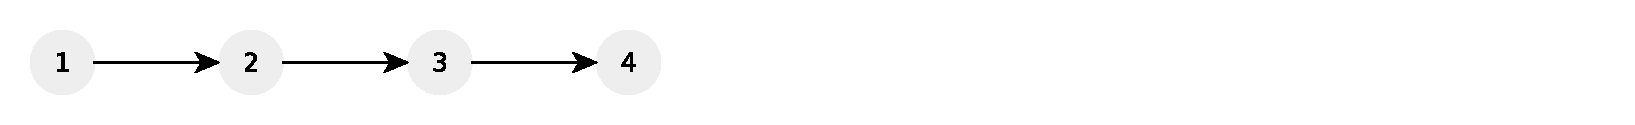
\includegraphics[width=1\linewidth]{sources/delete_duplicates_list/images/example2_2}
		  \caption{List shown in Figure \ref{fig:delete_duplicates_list:example2_1} with duplicates removed.}
		  \label{fig:delete_duplicates_list:example2_2}
	   \end{subfigure}
	 \caption[]{Input and output for the Examples \ref{ex:delete_duplicates_list:example1} and \ref{ex:delete_duplicates_list:example2}}
	  \label{fig:delete_duplicates_list:example1}
\end{figure}



\begin{lstlisting}[language=c++, caption=Singly Linked list definition,label=list:delete_duplicates_list:linked_list]
template<typename T>
struct Node {
	T val;
	Node *next;
	Node(T x) : val(x), next(nullptr) {}
};
\end{lstlisting}

\section{Clarification Questions}

\begin{QandA}
	\item \begin{questionitem} \begin{question} Can the input list be modified?  \end{question} 	 
    \begin{answered}
		\textit{Yes.}
	\end{answered} \end{questionitem}

	\item \begin{questionitem} \begin{question} Is it guaranteed the input list to be a valid list?  \end{question} 	 
		\begin{answered}
			\textit{The input list is always a valid singly linked list.}
		\end{answered} \end{questionitem}
	
\end{QandA}

\section{Discussion}
\label{delete_duplicates_list:sec:discussion}
There are several approaches to solving this problem but we will focus on two, the second of which is a refinement of the first intended to allow you to present an elegant and efficient solution in a short time frame.

\subsection{Brute-force}
\label{delete_duplicates_list:sec:bruteforce}
The easiest solution possible is as follows:
\begin{enumerate}
	\item Create a vector that contains a copy of the list
	\item Remove duplicates from the vector
	\item Create a new List with the content of the duplicate free vector
\end{enumerate}
This solution is straightforward but not optimal as, while it is optimal in time we are not taking advantage of the fact that we can modify the list in place and thereby avoid creating and returning a brand new list.  

A possible implementation is shown in Listing \ref{list:delete_duplicates_list_brite_force1} where for the step $2$ the  remove-erase idiom\cite{cit::wiki::remove-erase} is used to remove duplicates from the vector(the erase part is actually not necessary in this case).

\lstinputlisting[language=c++, caption={C++ solution $O(n)$ time and $O(n)$ space solution to the problem of removing duplicates from a Linked List using std::remove.},label=list:delete_duplicates_list_brite_force1]{sources/delete_duplicates_list/delete_duplicates_list_solution1.cpp}


\subsection{In-place $O(1)$ space solution}
\label{delete_duplicates_list:sec:linear_space}
In the solution describe in Section \ref{delete_duplicates_list:sec:discussion} used additional space to both remove the duplicates and also to avoid the pain of rearranging the input list by creating a brand new list containing no duplicates. It is, however,  possible to write a in-place solution that uses no additional space. 

The main idea is that since the list is \textbf{sorted}, duplicate elements will be one after the other. We can take advantage of this by simply ignoring pairs of consecutive nodes that have the same payload. Ignored nodes can therefore be deleted. The only complications is that we need to make sure to connect the first occurrence of every Node in the list with each other. It is f or this reason that we need to remember the first Node of a stride of the same value.

This idea is demonstrated in Listing \ref{list:delete_duplicates_list_lineartime}. Note that:

\begin{itemize}
	\item[-] The base case \lstinline[columns=fixed]{if(!head || !head->next) return head;} is making sure that if we are examining the last element of the list (or an empty list) then there is no duplicate to ignore and thus we can return this element.
	\item[-] otherwise, we are looking at a list with \textbf{at least} two elements. These two elements can be potentially the start of a stride of equal elements that we want to ignore. We keep a pointer,\lstinline[columns=fixed]{Node<T>* head;} (which is never modified) to the first element  of the stride and advance a second pointer, \lstinline[columns=fixed]{Node<T>* head_n;}, until we either reach the end of the list or we find an element that is different from the first one, \lstinline[columns=fixed]{while ( head_n && head -> val == head_n -> val)}. All the advanced elements are deleted. At the end of the loop the second pointer  is pointing to either:
	\begin{itemize}
		\item[-] An element different from the element pointed to  by the first one. The stride of equal elements is processed and  \lstinline[columns=fixed]{head->next} can now point to the second pointer.
		\item[-] \lstinline[columns=fixed]{nullptr}. We have reached the end of the input list. We are done.
	\end{itemize}
\end{itemize}


The time and space complexity for this approach are $O(n)$ and $O(1)$, respectively. All the nodes of the list are  visited at most once.

\lstinputlisting[language=c++, caption={C++ solution $O(n)$ time and $O(1)$ space solution to the problem of removing duplicates from a Linked.},label=list:delete_duplicates_list_lineartime]{sources/delete_duplicates_list/delete_duplicates_list_solution2.cpp}


\section{Common Variations and follow-up questions}
One follow-up question that an interviewer may ask relates to the deletion of the duplicate nodes. In the Listing \ref{list:delete_duplicates_list_lineartime} we see that the nodes are deleted using the \lstinline[columns=fixed]{operator delete}, but what if the list was not allocated using \lstinline[columns=fixed]{operator new}? The question is left for the reader.

\begin{exercise}
How would the solution change if the nodes were allocated using a custom allocator? (spoiler, a custom deleter is also needed.)
\end{exercise}